%%%%%%%%%%%%%%%%%%%%%%%%%%%%%%%%%%%%%%%%%%%%%%%%%%%%%%%%%%%%%%%%%%%%%%%%%%%
%% This file is part of the book
%%
%% Algorithmic Graph Theory
%% http://code.google.com/p/graph-theory-algorithms-book/
%%
%% Copyright (C) 2009--2011 Minh Van Nguyen <nguyenminh2@gmail.com>
%%
%% See the file COPYING for copying conditions.
%%%%%%%%%%%%%%%%%%%%%%%%%%%%%%%%%%%%%%%%%%%%%%%%%%%%%%%%%%%%%%%%%%%%%%%%%%%

\documentclass{article}

\usepackage{tikz}
\usetikzlibrary{external}
\tikzexternalize{5-2-Kneser-graph}

\begin{document}

\begin{figure}
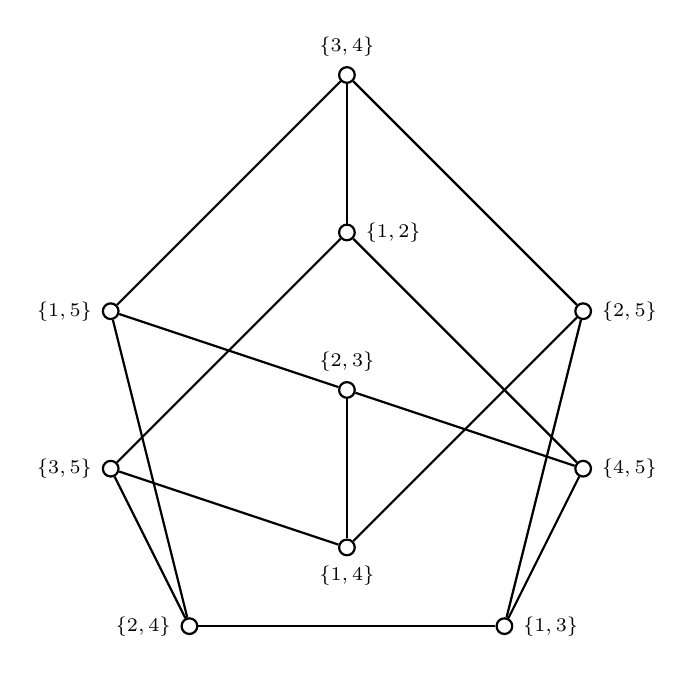
\begin{tikzpicture}
[lineDecorate/.style={-,thick},%
  nodeDecorate/.style={shape=circle,inner sep=2pt,draw,thick}]
%% nodes or vertices
\foreach \nodename/\x/\y in {
  24/0/0, 13/4/0, 15/-1/4, 25/5/4, 35/-1/2, 45/5/2, 14/2/1, 23/2/3,
  12/2/5, 34/2/7}
{
  \node (\nodename) at (\x,\y) [nodeDecorate] {};
}
%% node labels
\node [left] at (24.west) {\scriptsize$\{2,4\}$};
\node [right] at (13.east) {\scriptsize$\{1,3\}$};
\node [below] at (14.south) {\scriptsize$\{1,4\}$};
\node [left] at (35.west) {\scriptsize$\{3,5\}$};
\node [right] at (45.east) {\scriptsize$\{4,5\}$};
\node [above] at (23.north) {\scriptsize$\{2,3\}$};
\node [left] at (15.west) {\scriptsize$\{1,5\}$};
\node [right] at (25.east) {\scriptsize$\{2,5\}$};
\node [right] at (12.east) {\scriptsize$\{1,2\}$};
\node [above] at (34.north) {\scriptsize$\{3,4\}$};
%% edges or lines
\path
\foreach \startnode/\endnode in {
  24/13, 24/15, 24/35, 13/45, 13/25, 35/14, 35/12, 14/23, 14/25,
  45/23, 45/12, 15/23, 15/34, 34/12, 34/25}
{
  (\startnode) edge[lineDecorate] node {} (\endnode)
};
\end{tikzpicture}
\end{figure}

\end{document}
